\documentclass[10pt,twocolumn,a4paper]{article}
\usepackage[utf8]{inputenc}				% texto formato utf8
\usepackage{float}						% imagenes psosicion
\usepackage{cite}						% bibliografia
\usepackage[spanish,es-tabla]{babel}		% idioma
\usepackage{graphicx} 					% graficos 
\graphicspath{ {imagenes/} }				% path
\usepackage{multirow} 					% tablas
\title{\textbf{Cómo afecta el tamaño del problema y el número de procesos a la eficiencia de un algoritmo paralelo.}}
\author{Marlene E. Vásquez Calero}
\date{13 de Junio 2017}
\begin{document}
%-------------------------------------
%		PORTADA
%-------------------------------------
\begin{titlepage}	
	\begin{center}
	\begin{figure}
	\begin{center}
	
\includegraphics{aventur.jpg} \\ \
	\end{center}
	\end{figure}
	\begin{large}
	CURSO: \\ \ 
	$\LaTeX$  y Git aplicado a la investigación científica. \\ \
	\end{large}
	\vspace*{0.3in}			
	\rule{80mm}{0.1mm}\\ \
	\vspace*{0.1in}
	\begin{large}
	Profesores: \\
	Renato L. Ramirez Rivero \\
	Angel P. Hinojosa Gutiérrez\\
	\end{large}
	\end{center}
	\thispagestyle{empty}		% quitar numero de pagina	
\end{titlepage}
%-------------------------------------
\thispagestyle{empty} 			% quitar numero de pagina
%\pagestyle{empty}
\newpage	
$\ $

%-------------------------------------
\twocolumn[
	\begin{@twocolumnfalse}
	\maketitle
	\begin{abstract}
	\textit{ Se pretende demostrar por qué la eficiencia (E) tiende a aumentar al aumentar el tamaño del problema (N) y a disminuir al aumentar el número de procesos (P).}			
	\end{abstract}
	\begin{center}
	\rule{80mm}{0.1mm}\\ \
	\end{center}		
	\end{@twocolumnfalse}
]
%-------------------------------------
%		INTRODUCCION
%-------------------------------------
\section{Introducción}

El aprovechamiento del potencial de los sistemas paralelos requiere disponer de fundamentos de diseño e implementación de software paralelo, tanto para sistemas distribuidos como para sistemas paralelos de memoria compartida.\\
Ya que existen aplicaciones con elevados requisitos de cómputo que requieren software para plataformas multiprocesador.\\ Es por ello que se pretende demostrar por qué la eficiencia (E) tiende a aumentar al aumentar el tamaño del problema (N) y a disminuir al aumentar el número de procesos (P).
%-------------------------------------
%		DEMOSTRACION
%-------------------------------------
\section{Demostración}
%-------------------------------------
%		SUBSECTION
%-------------------------------------
\subsection{Modelo matemático}
Para demostrarlo se va a plantear un ejemplo y se utilizará el del \textbf{algoritmo del patrón de nueve puntos} \cite{Almeida2008} \textbf{la matriz tiene el mismo tamaño en todas las direcciones} (NxNxN). \\ Este algoritmo realiza operaciones sobre una matriz 3D y para computar cada punto hace falta conocer el valor de sus vecinos de arriba y abajo, dos a la izquierda, dos a la derecha, dos hacia delante y dos hacia atrás, además del propio punto (Figura \ref{fig:nuevePuntos}).
\begin{figure}[H]
\begin{center}
	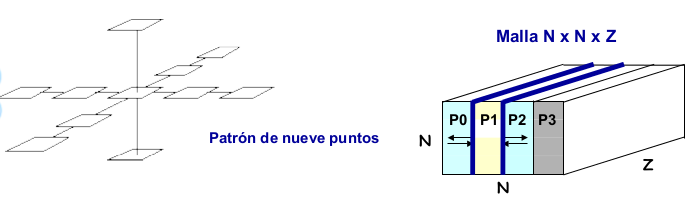
\includegraphics[height=2cm, width=6cm]{nuevePuntos}
	\caption{Patrón de nueve puntos, tamaño de la malla y reparto de ésta entre los procesos}
	\label{fig:nuevePuntos}
	\end{center}
\end{figure}
El tiempo de un algoritmo secuencial sería ($T_{1}$):
\begin{equation}
	T_{1} = t_{c}N^{3}
\end{equation}

Cuando se paraleliza, se reparten bloques de la matriz como se muestra en la Figura \ref{fig:oncePuntos}, por tanto cada proceso necesitará intercambiar $2N^{2}$ puntos con dos vecinos. Lo que hace que el tiempo de comunicación ($T_{comm}$) sea:
\begin{equation}
	T_{comm} = 2(t_{s} + t_{w}2N^{2})
\end{equation}

Y el tiempo de computación ($T_{comp}$):
\begin{equation}
	T_{comp} = \frac{t_{c}N^{3}}{P} 
\end{equation}

Por tanto el tiempo del algoritmo paralelizado ($T_{p}$) sería:
\begin{equation}
	T_{p} = T_{comp} + T_{comm} = \frac{t_{c}N^{3}}{P} + 2t_{s} + t_{w}4N^{2}
\end{equation}

La ganancia de velocidad (S) se calcula como la división del algoritmo secuencial ($T_{1}$) entre el paralelo ($T_{p}$):
\begin{equation}
	S = \frac{T_{1}}{T_{p}} = \frac{t_{c}N^{3}}{\frac{t_{c}N^{3}}{P} + 2t_{s} + t_{w}4N^{2}}
\end{equation}
Y la eficiencia (E), finalmente, se calcularía como la división entre la ganancia de velocidad (S) entre el número de procesos (P):
\begin{equation}
	E = \frac{S}{P} = \frac{t_{c}N^{3}}{P( \frac{t_{c}N^{3}}{P} + 2t_{s} + t_{w}4N^{2})}
\end{equation}

En esta función resultante contamos con cinco variables:
\begin{itemize}
	\item $t_{c}$: tiempo de computación por punto.
	\item $t_{s}$: tiempo de inicialización de comunicación.
	\item $t_{w}$: tiempo de comunicación por palabra.
	\item N: tamaño de la matriz.
	\item P: número de procesos.
\end{itemize}

Las tres primeras no varían, y se va a suponer que $t_{c}$ = 1 y $t_{s}$ = $t_{w}$ = 0.5. Por lo que vamos a utilizar la siguiente función para obtener los tiempos variando N y P:

\begin{equation}
	f(N,P) = \frac{N^{3}}{N^{3} + P + 2PN^{2}}
\end{equation}
%-------------------------------------
%		SUBSECTION
%-------------------------------------
\subsection{Mediciones y resultados}
Se toman tiempos con 1, 4, 8, 16 y 32 procesos y con tamaños de 64, 192, 320 y 512. Obteniendo los siguientes resultados: \\ \\

%tabla de datos
\begin{table}[H]
\begin{center}
\begin{tabular}{|l l l l l l|}
\hline
n&p=1&p=4&p=8&p=16&p=32\\
\hline
\hline
64		&1.0		&0.80	&0.57	&0.33	&0.17\\
192		&1.0		&0.92	&0.80	&0.60	&0.38\\ 
320		&1.0		&0.95	&0.87	&0.71	&0.50\\ 
512		&1.0		&0.97	&0.91	&0.80	&0.62\\ 
\hline
\end{tabular}
\caption{Datos}
\label{Tabla de datos}
\end{center}
\end{table}

\begin{figure}[H]
\begin{center}
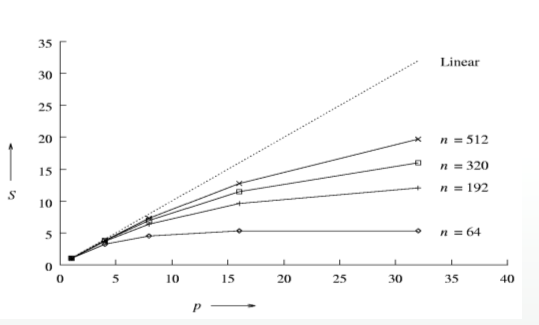
\includegraphics[height=4cm, width=5cm]{grafico}
\caption{La eficiencia disminuye conforme se aumenta el número de procesos}
\end{center}
\end{figure}

%-------------------------------------
%		CONCLUSION
%-------------------------------------
\section{Conclusión}
La eficiencia se define como la \textbf{fracción de tiempo en el que los procesos realizan un trabajo útil}.\\ \\
Por ello, es obvio pensar que a más procesos, más tiempo de comunicación y, por tanto, menos tiempo de trabajo útil. Los resultados obtenidos son coherentes respecto a esta afirmación y podemos ver como para todos los tamaños, la eficiencia disminuye.\\ \\
Al mismo tiempo, se puede presuponer que, de acuerdo a la definición que se da de eficiencia, al aumentar el tamaño del problema más carga de trabajo útil tendrán los procesos y por tanto mayor  será el porcentaje de su tiempo dedicado a ello .
%-------------------------------------
%		BIBLIOGRAFIA
%-------------------------------------
\bibliography{bibliografia}
\bibliographystyle{plain}
\end{document}